\chapter{Linear Kinetics}
\label{chapter:linear_kinetics}
Some of the contents of this chapter are reprinted, with permission, from \
\begin{enumerate}
\item[\cite{ch4_10_bai2016sum}] Bai, S., \& Skodje, R. T. The Sum Over Histories Representation for Chemical Kinetics: A Quantitative Theory Based on Chemical Pathways. \textit{International Reviews in Physical Chemistry}, 35(4), 539-567. \textbf{2016}
\end{enumerate}
\section{Analytical Expression of Linear Kinetics}
\label{ch2dot5:sec:analytical}
If the chemistry of a system is accurately described by a purely linear kinetic model,
then the implementation of the SOHR becomes especially simple. We use this transparent
case to illustrate some of the characteristics of the method. Consider a reaction network
consisting of N-species, $S_i$ $(i = 1, \cdots, N)$, which can undergo the first-order
reactions $S_i \xrightarrow[]{} S_j$ described by the rate laws $k_{i,j}[X_i]$. The graph for this linear system is
'simple' since at most one edge (reaction) will connect any two vertices (species) and
there are no self reactions, $S_i \nrightarrow S_i$. Thus, any n-step path can be uniquely represented
by the corresponding product of species, $S_0S_1 \cdots S_n$ and it is not necessary to specify
the reactions. The quantities $A_{i,j}(t)$ defined in eqn. \ref{ch2:eqn11} are constants in time, i.e.
$A_{i,j}(t) = k_{i,j}$. The species decay rates, $A_i = \sum{A_{i,j}} = \sum{k_{i,j}} \equiv k_i$, are likewise time-independent
and all the species survival probabilities correspond to pure exponential decay, i.e.
${\mathcal{P}}_{i}(t_a, t_b)=exp\left(-k_i(k_a-k_b)\right)$. The reaction branching ratios are given by $\Gamma_i=k_{i,J}/k_i$ where
$J$ denotes the appropriate channel along the pathway selected. Thus, for linear kinetics
the reference trajectory $\mathbf{X}(t)$ from eqn. \ref{ch2:eqn2} is not required to implement the
SOHR. Given these simplifications, the integral of the time-ordered product, eqn. \ref{ch2:eqn3}, can then be evaluated analytically\cite{ch1_IRPC_16_ch3_6_ch4_8_bai2014sum}
\begin{eqnarray}
  \twochoices
	{P_{path} \left(t_0, t_f \right) = \sum_{i=0}^{n}{D_i^n exp \left( -k_i(t_f - t_0) \right)}, && (a)}
	{D_i^n = \frac{\prod_{j=0}^{n-1}{k_j\Gamma_j}}{\prod_{j=0,j \neq i}^{n}{ \left( k_i - k_j \right) }}, && (b)}
\label{ch2dot5:eqn1}
\end{eqnarray}
The pathway probability is seen to be related to the integrated rate law for n-sequential
first-order reactions.\cite{ch1_IRPC_47_abel1906besonders} We note that the apparent singularity of this expression, which
occurs when two decay rates are equal, $k_i = k_j$, can be removed by making a small displacement
of one of the $k_i$'s.
\newline
\paragraph{}
\begin{figure}[htbp]
	\caption[Chemical graph corresponding to an acyclic linear kinetic model]{The chemical graph corresponding to an acyclic linear kinetic model with 5 species.
The edges connect only the species $S_i \xrightarrow[]{} S_j$ with $j > i$.}
    \begin{center}
	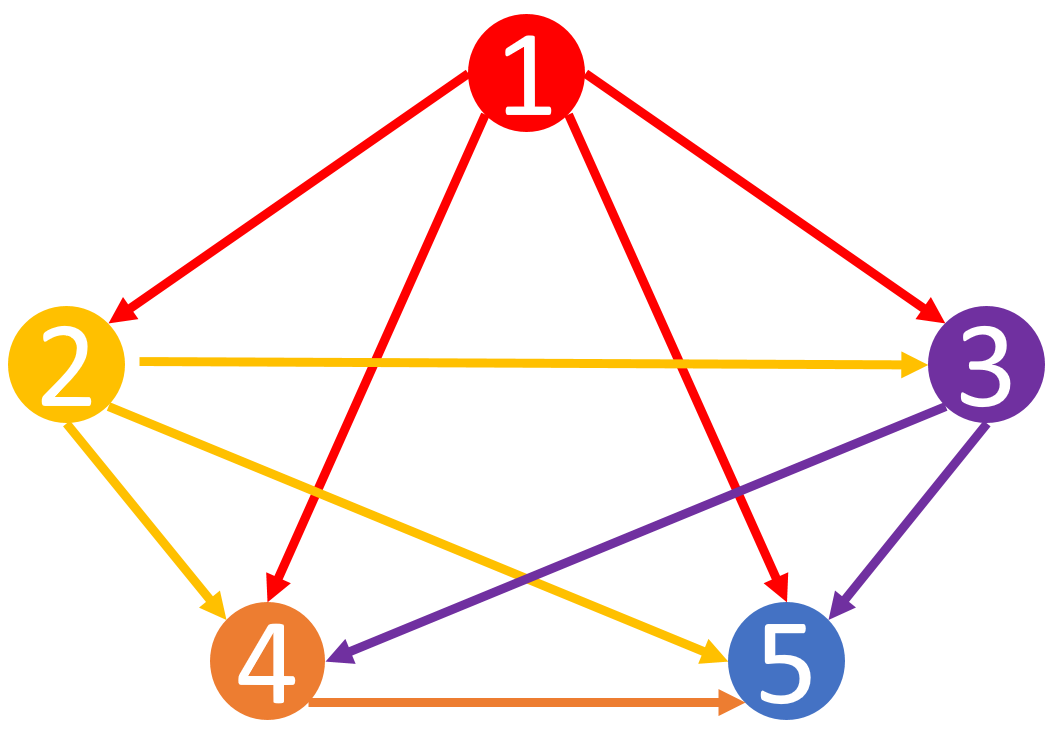
\includegraphics[width=100mm]{figs/chapter2dot5/fig2.png}
    \end{center}
\label{ch2dot5:fig2}
\end{figure}
To illustrate the workings of the SOHR for linear kinetics, we consider a simple 20
species system, i.e. $N = 20$, where the graph is acyclic. In an acyclic graph, no path
can form a closed loop and thus all the paths are of finite length. This condition is
enforced here by the condition $k_{i,j} = 0$ when $i \geq j$. In Fig. \ref{ch2dot5:fig2} we show the chemical
graph restricted to the first 5 species. We allow the lower triangle of the rate constant
matrix $k_{i,j}$ to be fully occupied. The non-zero rate constants are selected with a random
number generator over an order of magnitude range, i.e.
\begin{equation*}
k_{i,j} = 1 + \left( 10 - 1\right) \times random \left(0,1 \right)
\end{equation*}
We find most random sets of rate constants give results that are qualitatively similar.
\section{Number of Pathway vs. Pathway Length}
\label{ch2dot5:sec:path_len}
Using the adjacency matrix, eqn. \ref{ch2:eqn17}, we find that the number of potential
pathways can grow quite large even for this simple problem. For example, if we follow
species $S_1$ through the network to species $S_{20}$ there are $262,144$ allowed paths that a
molecule might take. In Fig. \ref{ch2dot5:fig3}, we show the distribution of paths vs. path length, $L$.
There is one path of length $L = 1$, viz. $S_1 \xrightarrow[]{} S_{20}$, and one path of length $L = 19$, viz.
$S_1 \xrightarrow[]{} S_2 \cdots → S_{19} \xrightarrow[]{} S_{20}$. The largest number of paths occur in the middle of the
range, $L = 10$. Of course the number of paths will depend on the choice of initial and
final species.
\begin{figure}[htbp]
	\caption[Number of path and path length distribution of linear model]{The number of independent chemical pathways connecting species $S_1$ with $S_{20}$ in a
linear kinetic model with rate coefficients $k_{i,j} \neq 0$ for $j > i$ and $k_{i,j} = 0$ for $i \geq j$. The length $L$ is
the number of reactions along the path.}
    \begin{center}
	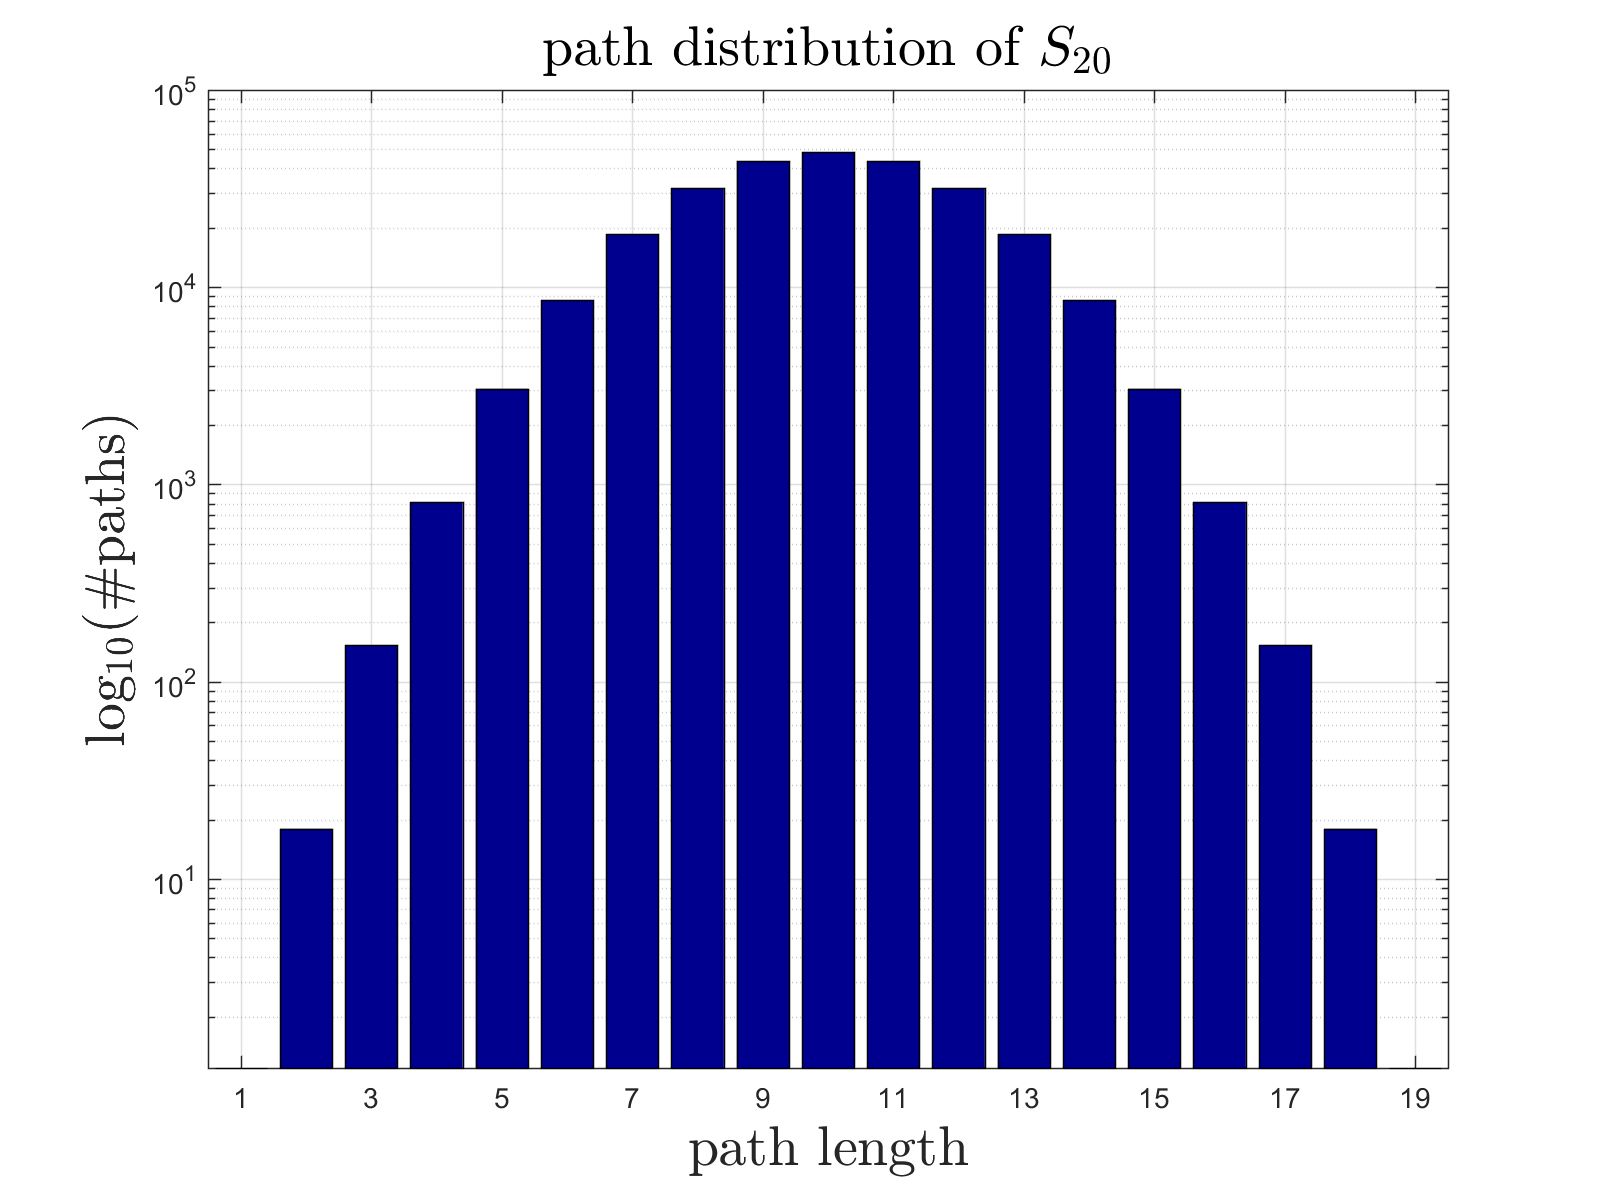
\includegraphics[width=100mm]{figs/chapter2dot5/fig3.png}
    \end{center}
\label{ch2dot5:fig3}
\end{figure}
\section{Demonstration of Convergence of SOHR}
\label{ch2dot5:sec:convergence}
In order to assess the numerical performance of the SOHR method, we have
computed for comparison the 'exact' solution to the linear system using a 4th-order
Runge-Kutta integration of the differential kinetics equations
\begin{eqnarray}
\label{ch2dot5:eqn2}
\frac{d [X_i]}{dt} = Sources - Sinks = \sum_{j=1}^{i-1}{k_{i,j}[X_j] - k_i[X_i]}
\end{eqnarray}
We note that species $S_{20}$ is stable since $k_{20} = 0$. Thus, for the initial condition
$[X_i(t = 0)] = \delta_{i,1}$ we know that the solution will tend to $[X_{20}(t)] \rightarrow 1$ as $t \rightarrow \infty$. We
shall compare the Runge-Kutta solution of the kinetics originating from the $S_1$ initial
condition to the prediction of the SOHR using the pathways originating with $S_1$. We
note that if all the chemical paths are included in the SOHR expansion we also obtain
the exact result.
\newline
\paragraph{}
Using the stochastic method described in Section \ref{ch2:sec:Stochastic_pathway_enumeration}, we have identified a number
of candidate pathways that converts species $S_1$ to each of the other species, $S_i$. Thus,
we have run several thousand MC trajectories and produced a rough ranking of the pathways that connect $S_1$ to the other species.
In Fig. \ref{ch2dot5:fig4}, we show the concentrations
of several intermediate species computed using eqn. \ref{ch2dot5:eqn1} and the pathway expansion $ \left[ X_i(t_f) \right] = \sum_{j}{P_j \left[ X_1 \right] }$. To achieve better than 1$\%$ accuracy, we used 8 paths for $S_5$, 25 paths for $S_{10}$, and 300 paths for $S_{15}$. Clearly, the pathway representation
reaches practical convergence for the concentration long before the all of the
potential paths are included. Indeed, the rapid convergence of the expansion with
respect to the number of paths is a criterion for the practical utility of the SOHR as a
computational method.
\begin{figure}[htbp]
	\caption[The concentration from SOHR vs. concentration from ODEs]{The concentration of several chemical intermediates vs. time for the linear kinetic
model consisting of 20 species. The solid lines are the result of converged numerical integration
of the conventional kinetics equations, eqn. \ref{ch2dot5:eqn2}, for species $S_5$, $S_{10}$, and $S_{15}$. The symbols
are the result of the SOHR using eqn. \ref{ch2dot5:eqn1} for the pathway probabilities. The pathways
were identified using a small stochastic simulation.}
    \begin{center}
	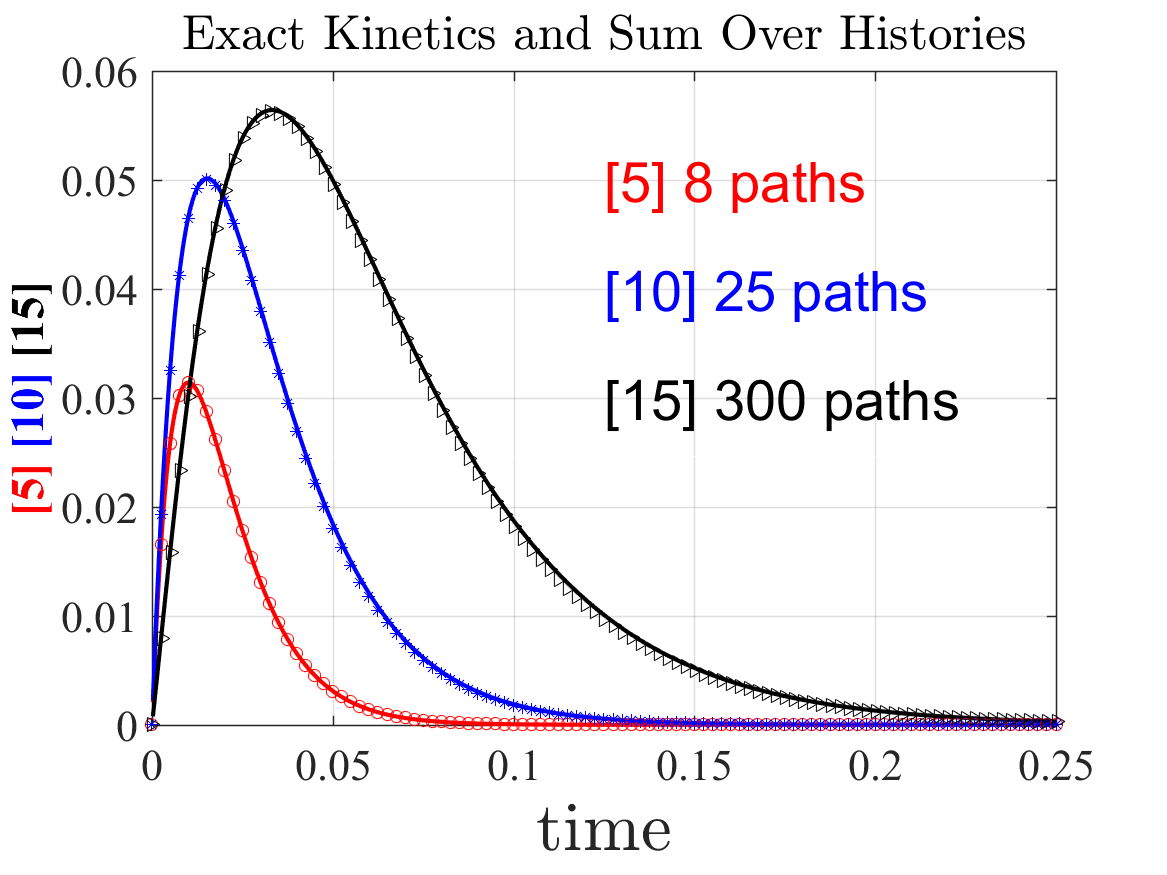
\includegraphics[width=100mm]{figs/chapter2dot5/fig4.png}
    \end{center}
\label{ch2dot5:fig4}
\end{figure}
\section{Pathway Probabilities Changing Over Time}
\label{ch2dot5:sec:p_prob_time}
It is instructive to investigate the behaviour of the SOHR in somewhat greater detail
for this simple problem. We note that even though the pseudo-first-order rate coefficients
are time-independent, the pathway probabilities still possess a strong time-dependence.
In Fig. \ref{ch2dot5:fig5}, we show the pathway probabilities vs. time for the 100 most
important paths connecting $S_1$ to $S_{15}$. The paths are colour-coded according to their
length. At very early times, the one-step path, i.e. $S_1 \xrightarrow[]{} S_{15}$, dominates the probability.
At somewhat later times, the two-step paths, i.e. $S_1 \xrightarrow[]{} S_j \xrightarrow[]{} S_{15}$ begin to play a role.
At still later times, the three- and four-step paths begin to contribute. Heuristically, we can understand that a molecule which arrives at species $S_{15}$ at a later time will tend to take a more circuitous route than one that arrives at an earlier time. In Fig. \ref{ch2dot5:fig6}, we
show the growth of the mean path length as a function of time. Obviously the concentration
of a kinetic intermediate is closely connected to the notion of arrival time distributions
or first passage time distributions that are often studied in stochastic models.\cite{ch1_IRPC_33_van1992stochastic} If we consider the full passage through the network to the attracting final state,
$S_{20}$, the pathway probabilities take a simple form. As $t \rightarrow \infty$, the sum of exponentials in eqn. \ref{ch2dot5:eqn1} contains only the last term with $k_{20} = 0$. In this case, the pathway
probability becomes the product of the branching ratios along the path and is time-independent.
It is interesting to point out that even for a general non-linear mechanism, if
the kinetics reaches a steady state condition then the same linear analysis may be
invoked to implement the SOHR.
\begin{figure}[htbp]
	\caption[Pathway probabilities vs. time]{Pathway probabilities vs. time for the 100 most probable paths connecting $S_1$ with $S_{15}$
in the linear kinetic model. At each time, the sum of probabilities is normalised to unity. The
pathway probabilities are colour coded according to their path lengths.}
    \begin{center}
	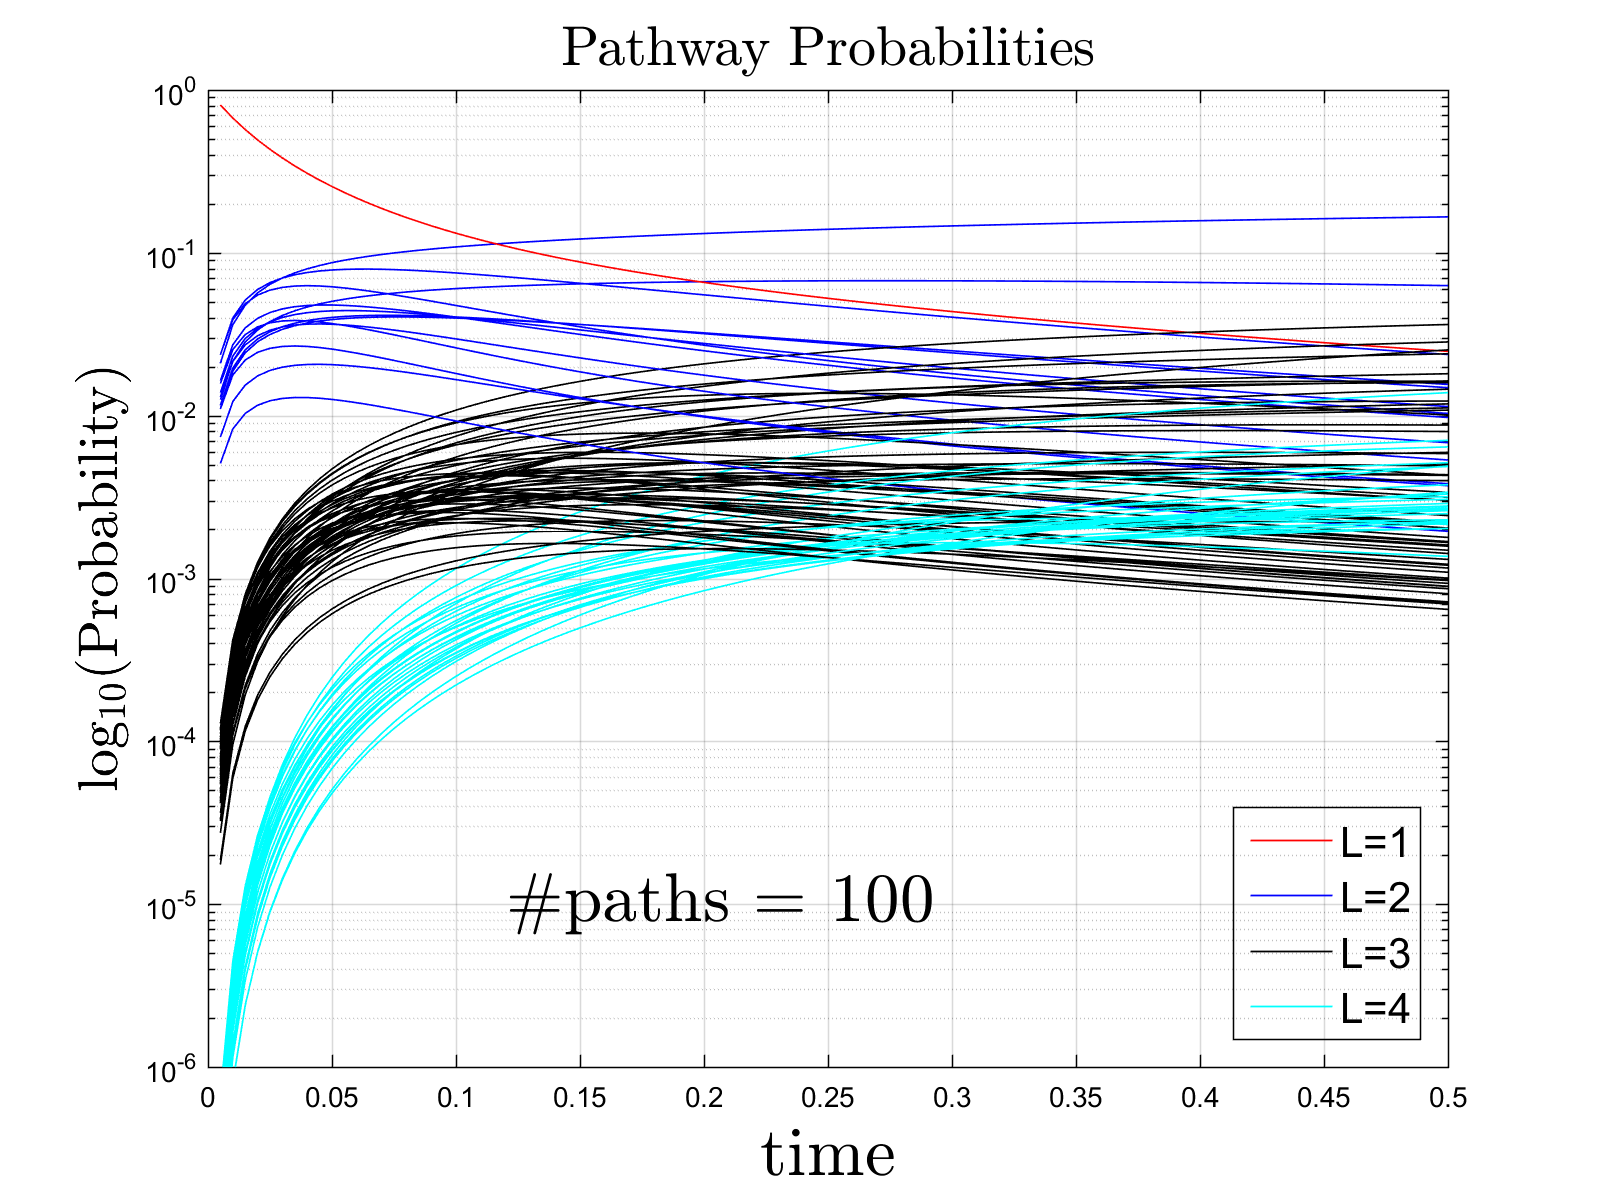
\includegraphics[width=100mm]{figs/chapter2dot5/fig5.png}
    \end{center}
\label{ch2dot5:fig5}
\end{figure}
\begin{figure}[htbp]
	\caption[The average path length vs. time]{The average path length vs. time for chemical paths going from S1 to S15 in the linear
kinetic model. The weight of each chemical path is computed using Equation (3.1) where the
weights are normalised to unity at each time.}
    \begin{center}
	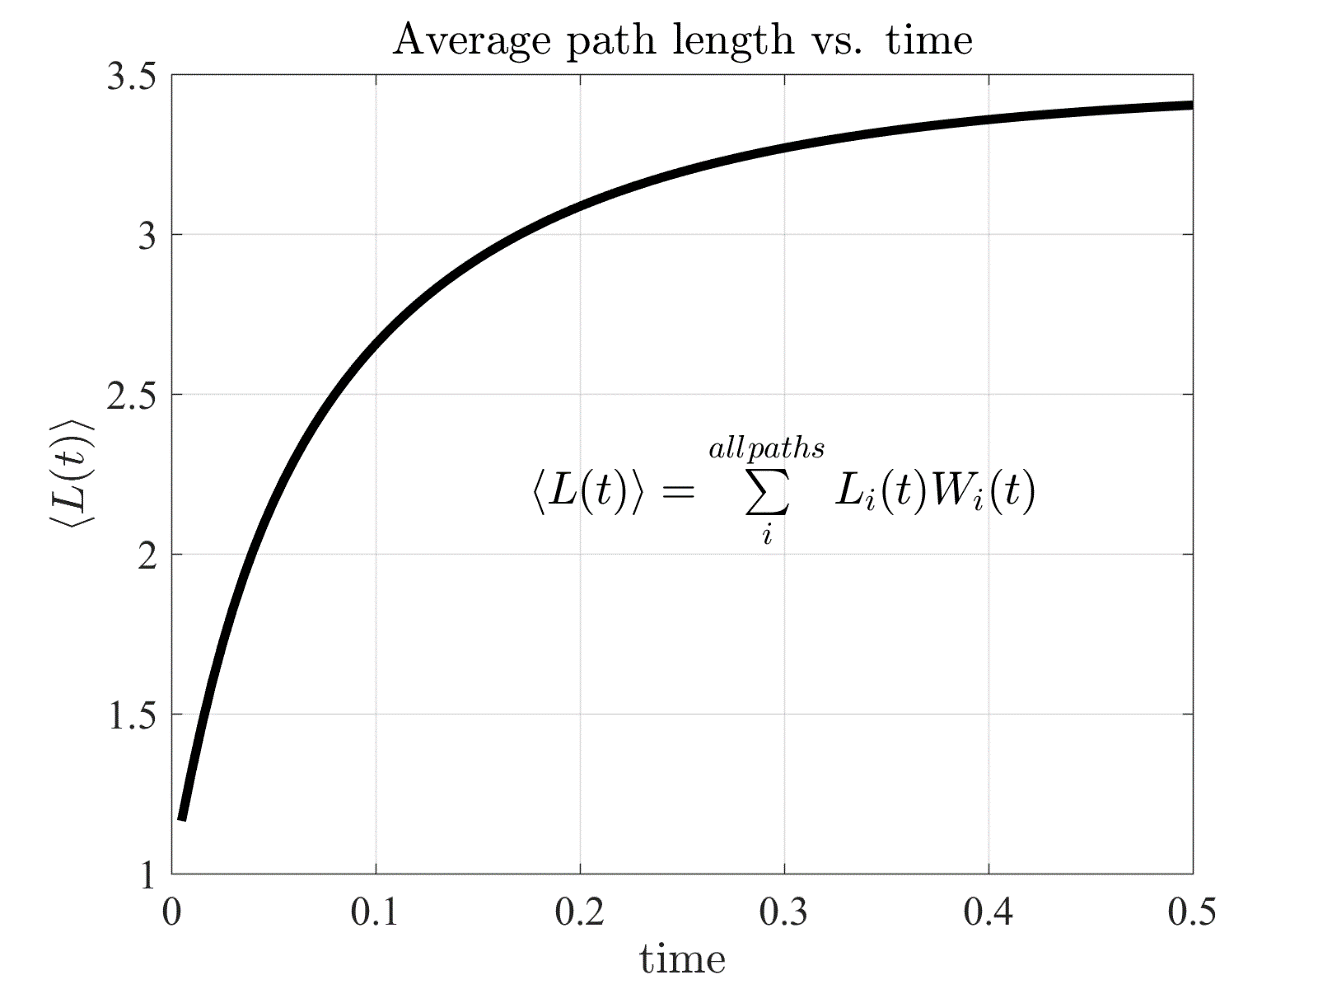
\includegraphics[width=100mm]{figs/chapter2dot5/fig6.png}
    \end{center}
\label{ch2dot5:fig6}
\end{figure}